\section{Data and preprocessing}
\label{app:preprocessing}

\paragraph{Data split.}
MOSTA supplies 53 mouse embryo sections. We reserved one section from each developmental stage from E9.5 to E16.5 in advance for evaluation and used the remaining 45 sections for pretraining. Training spans the same eight stages. Table~\ref{tab:heldout-inventory} lists the held-out sections; Table~\ref{tab:evaluation_protocol} summarizes data use and aggregation for each analysis.

\begin{table}[!htbp]
\centering\small
\caption{\textbf{Held-out section inventory.} Every listed section is excluded from both pretraining stages.}
\label{tab:heldout-inventory}
\begin{tabular}{ll}
\toprule
Stage & Held-out section \\
\midrule
E9.5 & E9.5 E2S4 \\
E10.5 & E10.5 E2S1 \\
E11.5 & E11.5 E1S4 \\
E12.5 & E12.5 E2S1 \\
E13.5 & E13.5 E1S4 \\
E14.5 & E14.5 E2S2 \\
E15.5 & E15.5 E2S1 \\
E16.5 & E16.5 E2S13 \\
\bottomrule
\end{tabular}
\end{table}

\paragraph{Input preprocessing.}
The inputs use the original \texttt{count} layer and a 30,235-entry gene vocabulary. Existing center tokens are inherited from the prepared source data. Neighborhood profiles average normalized expression over the full gene space before selecting up to 512 tokens and assigning 31 nonzero expression bins, with bin zero reserved for padding. The inherited preprocessing uses library normalization to $10^4$, $\log(1+x)$, and section-specific nonzero gene medians; genes with fewer than ten nonzero observations use a fallback median. Target sections supply their own gene statistics and use the inherited vocabulary. Whole-section readout standardization, PCA, and clustering are fitted on target-section positions; method-specific settings are given in Appendix~\ref{app:dual-view}.

Relative coordinates are centered at the focal position and scaled by the maximum distance within its 128-neighbor window, then sliced to smaller supports. Granularity counts observations; its physical extent depends on the sampled tissue. Maps preserve the measured lattice and leave missing positions empty, without label interpolation.

\begin{table}[!htbp]
\centering\small
\caption{\textbf{Data split and evaluation protocol.} These conditions apply to the corresponding evaluations throughout the paper.}
\label{tab:evaluation_protocol}
\begin{tabularx}{\linewidth}{@{}p{0.20\linewidth}X@{}}
\toprule
Evaluation & Data use and aggregation \\
\midrule
Held-out sections & The eight sections in Table~\ref{tab:heldout-inventory} evaluate pretrained encoders with frozen weights. Input preprocessing and target-fitted readouts are specified above and in Appendix~\ref{app:dual-view}. \\
Anatomical analyses & E14.5 E1S1 (granularity and Facial nerve analyses) and E16.5 E1S1 (state and context-response analyses) belong to the training set. The E12.5 E2S1 whole-section map and E16.5 E2S13 Brain mapping display use held-out sections. \\
Developmental ordering & Stage-balanced Brain observations from the held-out sections evaluate pseudotime--stage agreement. Sampling, shared baseline fits, and both correlation readouts are specified in Appendix~\ref{app:developmental-ordering}. \\
Response summaries & Direct-encoding analyses use eight training E1S1 sections and eight holdouts. Section--domain--range summaries combine both groups; the high--low response comparison reports the eight holdouts separately. \\
Matched continuation & E12.5 E2S1, E14.5 E1S1, and E16.5 E1S1 are adapted separately and evaluated on the respective adapted section, using one training seed. E12.5 was excluded from base pretraining; the other two sections were included. \\
Aggregation & Section summaries receive equal weight. Position-level distributions describe within-section variation; queries, projections, shuffles and batches specify sampling and numerical averaging. \\
\bottomrule
\end{tabularx}
\end{table}

\paragraph{External pretrained models.}
Novae uses the public mouse-0 weights, and SToFM uses its public checkpoint with the specified mouse-to-human gene mapping. The sections held out from ZoomST training appear in the SToCorpus-88M inventory, so SToFM may have been exposed to our zero-shot evaluation data.

\section{Architecture and optimization}
\label{app:hyperparameters}

\subsection{Backbone and within-granularity learning}

Both representation views have width 256. The position-wise and pseudobulk encoders each use two Transformer layers and eight attention heads, with separate Transformer parameters and shared gene and expression-bin embeddings. The spatial-context Transformer has four layers and eight attention heads and is shared across granularities. The DeepSets maps $\phi$ and $\rho$ each use layer normalization and a two-layer multilayer perceptron with hidden width 512, GELU activation, and dropout 0.1. The same maps are applied at each granularity.

For clarity, the pooled profile and spatial set readout are
\begin{equation}
m_{i,r}=r^{-1}\sum_{j\in S_{i,r}}\bar x_j,\qquad
 g_{i,r}=\rho\!\left(r^{-1}\sum_{j\in S_{i,r}}\phi(H_{ij,r})\right).
\label{eq:neighborhood-profile}
\end{equation}
The base objective combines reconstruction with same-support view alignment:
\begin{equation}
\mathcal L_{\mathrm{base}}=\mathcal L_{\mathrm{rec}}+
\frac{\lambda_{\mathrm{view}}}{|\Rset|}\sum_{r\in\Rset}\mathcal L_{\mathrm{VICReg}}(e_r,g_r).
\label{eq:base-objective}
\end{equation}
Here $e_r,g_r$ collect the sampled centers at granularity $r$.

The molecular view averages preprocessed expression over the neighborhood before selecting up to 512 gene tokens and assigning expression bins. There are 31 nonzero expression bins and one padding bin. Reconstruction masks gene and value identities together at 30\% of visible nonzero token positions, with at most 154 queries per profile. A shared gene-bin decoder predicts the expression-bin targets, and only masked nonzero targets contribute to the reconstruction loss. With branch weights one,
\begin{equation}
\mathcal L_{\mathrm{rec}}
=\mathcal L_{\mathrm{center}}
+\frac{1}{|\Rset|}\sum_{r\in\Rset}
\left(\mathcal L_{g,r}^{\mathrm{PB}}+\mathcal L_{e,r}^{\mathrm{PB}}\right).
\label{eq:reconstruction-objective}
\end{equation}
The neighborhood losses reconstruct the pooled expression profile from the spatial and molecular states, respectively. Within-granularity VICReg is applied directly to these states, with invariance, variance, and covariance weights $(1,1,0.04)$ and outer weight $\lambda_{\mathrm{view}}=0.1$ in Equation~\ref{eq:base-objective}.

\subsection{Shared field and numerical integration}

For state $z\in\mathbb R^{256}$ and granularity coordinate $u$, the field is
\begin{equation}
f_\theta(z,u)
=W_2\,\operatorname{GELU}\!\left(
W_1[\operatorname{LN}(z);u]+b_1\right)+b_2,
\label{eq:ode-field-network}
\end{equation}
where $W_1\in\mathbb R^{128\times 257}$ and $W_2\in\mathbb R^{256\times 128}$. The field has 66,560 trainable parameters, including layer normalization. Both $W_2$ and $b_2$ are initialized to zero. The transition is evaluated in single precision, and gradients are propagated through the numerical integration steps.

For $u_a=u(a)$ and $u_b=u(b)$, integration uses uniform steps within each query interval, with $n=\max(1,\lceil |u_b-u_a|/0.25\rceil)$ and step size $h=(u_b-u_a)/n$. A zero-length interval returns its input. A fourth-order Runge--Kutta step from $(u,z)$ is
\begin{equation}
\begin{aligned}
k_1&=f_\theta(z,u),\\
k_2&=f_\theta(z+hk_1/2,u+h/2),\\
k_3&=f_\theta(z+hk_2/2,u+h/2),\\
k_4&=f_\theta(z+hk_3,u+h),\\
z^{+}&=z+\frac h 6(k_1+2 k_2+2 k_3+k_4).
\end{aligned}
\label{eq:rk4-transition}
\end{equation}
The training intervals $8\to 32$, $32\to 128$, and $8\to 128$ use two, two, and four steps, respectively.

The coordinate satisfies $u=\log_2(r/8)/4$, so the field per unit $\log_2 r$ is $f_\theta/4$. Equation~\ref{eq:granularity-response} uses the corresponding finite-interval normalization to compare response magnitudes across intervals of different widths.

\subsection{Coarse-support regression}

For a focal center $i$ and pair $(a,b)$, all $b$ positions in $S_{i,b}$ contribute a source state. Each state $e_{j,a}$ is encoded from the fine neighborhood centered at $j$. The observed target is $y=\stopgrad(e_{i,b})$, the current encoder's clean coarse state. Write $q_j=T_{a\to b}(e_{j,a})$ and $\bar q=b^{-1}\sum_{j\in S_{i,b}}q_j$. The loss for this support decomposes as
\begin{equation}
\frac{1}{bd}\sum_{j\in S_{i,b}}\|q_j-y\|_2^2
=\frac{\|\bar q-y\|_2^2}{d}
+\frac{1}{bd}\sum_{j\in S_{i,b}}\|q_j-\bar q\|_2^2.
\label{eq:consensus-decomposition}
\end{equation}
The cross term vanishes because $\sum_j(q_j-\bar q)=0$. Thus, the objective combines mean-to-target alignment and within-support prediction consensus. Every source is transformed before its error is computed. Losses are averaged within each support and then equally across focal centers and the three granularity pairs. The target is detached, while the predicted states carry gradients to the field and source encoder.

\subsection{Projected product-kernel MMD}

A fixed projection with orthonormal rows maps each 256-dimensional state to 16 dimensions and is stored with the model. For one granularity pair, define
\begin{equation}
s_i=\Pi\stopgrad(e_{i,a}),\qquad
q_i=\Pi T_{a\to b}(e_{i,a}),\qquad
t_i=\Pi\stopgrad(e_{i,b}).
\end{equation}
With the stop-gradient notation of the main text, the empirical joint measures are
\begin{equation}
\begin{aligned}
\widehat P_{ab}^{T,\Pi}
&=\frac{1}{B}\sum_{i=1}^{B}
\delta_{(\Pi\stopgrad(e_{i,a}),\,\Pi T_{a\to b}(e_{i,a}))},\\
\widehat P_{ab}^{\Pi}
&=\frac{1}{B}\sum_{i=1}^{B}
\delta_{(\Pi\stopgrad(e_{i,a}),\,\Pi y_{i,b})},
\end{aligned}
\label{eq:projected-joint-measures}
\end{equation}
where $\delta$ denotes a point mass. With $B$ focal-center samples, the biased empirical statistic used in Equation~\ref{eq:granularity-joint} is
\begin{equation}
\widehat{\operatorname{MMD}}_{ab}^{\,2}
=\frac{1}{B^2}\sum_{i,j=1}^{B}
\kappa_a(s_i,s_j)
\left[\kappa_b(q_i,q_j)+\kappa_b(t_i,t_j)
-2\kappa_b(q_i,t_j)\right].
\label{eq:empirical-joint-mmd}
\end{equation}
We use multibandwidth radial basis function kernels
\begin{equation}
\kappa_r(v,w)
=\frac{1}{3}\sum_{c\in\{0.5,1,2\}}
\exp\!\left(-\frac{\|v-w\|_2^2}{2 c^2\sigma_r^2}\right).
\label{eq:multibandwidth-rbf}
\end{equation}
The source bandwidth $\sigma_a^2$ is the median of positive pairwise squared distances among $s_i$, and the destination bandwidth $\sigma_b^2$ is computed from $t_i$. Bandwidths are detached, and the three granularity-pair statistics are averaged equally.

The source coordinate in the product kernel is held fixed during each gradient calculation. The prediction is computed from the full 256-dimensional source state before projection, so its gradients update the source encoder as well as the transition. Observed coarse states are clean, same-step outputs of the current encoder, detached as regression and MMD targets. The projected statistic is the empirical penalty used to optimize the joint relationship in Equation~\ref{eq:granularity-equivariance}.

\subsection{Joint optimization}

The reconstruction and view-alignment objective initializes the representations and remains active during cross-granularity training. Both relation coefficients are increased to one during warmup. All three source--target granularity pairs receive equal final weight. Encoder and transition parameters are optimized together; clean encodings supply the relation losses, while reconstruction is evaluated on masked inputs. Pretraining uses molecular measurements and spatial coordinates without anatomical labels.


For MOSTA, the base-pretrained encoder is followed by two joint-training epochs over 45 source sections, totaling 46,400 updates with a global batch of 160 (four devices, 40 centers per device). AdamW uses learning rates $2\times 10^{-4}$ for molecular and embedding parameters and $10^{-4}$ for the spatial context parameters, with respective weight decays 0.02, 0.01, and 0.05. Learning rates and the two relation weights warm up over 1,200 updates; cosine decay has a final learning-rate ratio of 0.1. Gradient norm is clipped at five. Backbone computation uses bfloat16 mixed precision and the ODE uses float32. Evaluation uses the final two-epoch checkpoint.

The No Cross ablation continues training from the epoch-10 base-pretrained initialization for 46,400 updates using reconstruction and within-granularity view alignment without cross-granularity supervision. Including the 161,810 base-pretraining updates, both No Cross and the full model receive 208,210 updates in total. Evaluation uses the completed continuation for each model.

For HESTA, all compared variants receive ten training epochs on the same 68 source sections: eight epochs with the base objective, followed by two epochs with each variant's objective. ZoomST adds coarse-support regression and JointMMD during the final two epochs; No Cross continues with reconstruction and within-granularity view alignment. Evaluation uses each variant's final ten-epoch model.

The HESTA ZoomST continuation uses a global batch of 672 (eight devices, 84 centers per device). AdamW uses learning rates $2\times10^{-4}$ for molecular and embedding parameters and $10^{-4}$ for spatial context parameters, with respective weight decays 0.02, 0.01, and 0.05; normalization and bias terms receive no weight decay. Learning rates and the two relation weights warm up over 500 updates, followed by cosine learning-rate decay to a final ratio of 0.1. Gradient norm is clipped at five. Backbone computation uses bfloat16 mixed precision and the ODE uses float32.


\section{Tissue representation evaluation}
\label{app:scale-cases}

\subsection{Anatomical granularity cases}

The anatomical granularity analysis uses E14.5 E1S1 and the frozen MOSTA model defined in Section~\ref{sec:experiments}. Its 102,519 measured positions supply neighborhood context; scoring uses the fixed union of Heart (2,952), Lung (2,011), Liver (6,015), GI tract (1,260), Smooth muscle (1,737), and Pancreas (425). Each output is standardized and projected by full-SVD PCA 32 on these 14,400 positions. MiniBatchKMeans uses six clusters, batch size 2,048, three initializations, at most 200 iterations, no-improvement limit 30, and seed 42. Atlas annotations define the domain, cluster count, post-hoc maximum-overlap one-to-one assignment, and scores. They do not fit the feature transform or clustering.

Scores are computed over all positions in the fixed evaluation domain. The maps preserve measured coordinates without smoothing or interpolation. Coarse and fine maps share viewing limits and the same readout settings.

For class $c$, predicted and annotated position sets $P_c,T_c$ within the fixed scoring domain define
\begin{equation}
\mathrm{IoU}_c=\frac{|P_c\cap T_c|}{|P_c\cup T_c|}
=\frac{\mathrm{TP}_c}{\mathrm{TP}_c+\mathrm{FP}_c+\mathrm{FN}_c}.
\label{eq:iou}
\end{equation}
TP counts correct assignments, FP extra assignments, and FN missed targets.

Adjusted mutual information (AMI) measures the information shared by cluster and annotation assignments after subtracting chance mutual information and dividing by mean marginal entropy minus that same chance expectation. The adjusted Rand index (ARI) measures chance-corrected agreement in whether pairs of positions share a class. Both are invariant to cluster renaming.

\subsection{Whole-section tissue mapping and neighbor retention}
\label{app:dual-view}

The tissue-mapping evaluation uses the MOSTA and HESTA held-out sections listed in Appendix~\ref{app:preprocessing}. Both atlases include cross-method comparisons and the granularity-specific No Cross comparison. ZoomST and public pretrained encoders remain frozen; target-fitted methods are identified separately.

The equal-budget controlled ablation compares the final ZoomST and No Cross checkpoints after the same total number of training updates within each atlas; No Cross omits cross-granularity supervision. Both models use the same joint readout and are frozen during evaluation. Optimization and update budgets are specified in Appendix~\ref{app:hyperparameters}.

The displayed Molecular View, Spatial View, and Joint refer to three readouts of the same frozen ZoomST model. Molecular features concatenate the three 256-dimensional outputs $e_8,e_{32},e_{128}$; spatial features concatenate $g_8,g_{32},g_{128}$. Joint features concatenate all six outputs. For MOSTA, Novae uses its public mouse-0 checkpoint; SToFM uses its public checkpoint with the declared mouse-to-human gene mapping. Each ZoomST or public pretrained candidate is independently standardized and projected to 32 dimensions using randomized PCA with seed 42, 32 oversamples, five power iterations, and no whitening. Standardization and PCA fit all eligible target-section positions without annotation values. MiniBatchKMeans uses $K$ clusters, where $K$ is the number of classes in the section's primary MOSTA \texttt{annotation} field or HESTA coarse \texttt{celltype} field, with k-means++ initialization, ten initializations, batch size 4,096, at most 300 iterations, a ten-step no-improvement limit, and seeds 42, 43, and 44.

Scores use the same eligible positions for every method within each benchmark: all positions for MOSTA and the common valid cohort specified below for the HESTA cross-method comparison. Adjusted mutual information (AMI) and adjusted Rand index (ARI) measure chance-adjusted agreement between the cluster partition and the atlas annotation. One-to-one maximum-overlap Hungarian matching assigns anatomical labels to clusters for the maps and class-specific IoU. For class $c$, $\operatorname{IoU}_c=\operatorname{TP}_c/(\operatorname{TP}_c+\operatorname{FP}_c+\operatorname{FN}_c)$. AMI and ARI are invariant to the matching. Section-level scores are averaged with equal section weights.

\paragraph{Target-fitted spatial methods.}
GraphST, BANKSY, MENDER, and STAGATE~\citep{long2023graphst,singhal2024banksy,yuan2024mender,dong2022stagate} use each complete target section independently, with expression and coordinates but no anatomical training labels. Each fixed representation uses the shared clustering protocol above. Tables group these target-fitted methods separately from frozen pretrained representations.

GraphST and STAGATE select 3,000 highly variable genes by Seurat-v3 on raw counts, followed by counts-per-10,000 normalization and log1p. GraphST additionally applies noncentered gene scaling clipped at 10. GraphST uses its Stereo-seq three-neighbor graph and a sparse implementation of the native objective, with 600 epochs, learning rate 0.001, and hidden dimension 64. The readout uses its normalized reconstructed-gene output. STAGATE uses the official PyG model, a symmetrized six-neighbor graph with self loops, hidden dimensions 512 and 30, 1,000 epochs, learning rate 0.001, weight decay 0.0001, and gradient clipping at 5. It uses the full section graph without an annotation-derived auxiliary graph.

BANKSY and MENDER normalize all genes to counts per 10,000, apply log1p, and select 3,000 genes by Seurat dispersion. BANKSY uses neighborhood statistics with 15 and 30 neighbors for orders zero and one and scaled-Gaussian decay. The fixed primary weight is $\lambda=0.8$, the official default for tissue-domain segmentation~\citep{singhal2024banksy}; the documentation explicitly includes Stereo-seq among the technologies for which this setting is recommended.\footnote{\url{https://prabhakarlab.github.io/Banksy/}, accessed 15 September 2026.} BANKSY's native channel normalization and weighting are preserved, without a second StandardScaler before PCA32. MENDER derives 32 unsupervised expression states using StandardScaler, PCA32, and MiniBatchKMeans with ten initializations; it then aggregates these states over six rings with ring parameter four, including the center, producing 192 features. MENDER's state labels are independent of the anatomical annotation.

The shared randomized-PCA and clustering settings above apply to these features. STAGATE retains its native 30 dimensions; the other methods use PCA32. The comparison shares positions, labels, and downstream algorithms while retaining these method-specific feature definitions.

\paragraph{Human cross-method benchmark.}
Table~\ref{tab:hesta-representation-summary} uses the independently pretrained human ZoomST model and seven HESTA sections. All methods share 1,129,281 positions with valid representations, excluding six positions outside the common cohort. Novae uses its public human-0 checkpoint with native count normalization, log1p, and unlabeled per-section gene selection and scaling. SToFM uses human gene names directly. scGPT-spatial normalizes raw expression by the whole-section matched nonzero mean and pretrained gene means. TERRA~\citep{birk2026terra} provides Cell, Neighborhood, and Spatial-cell outputs using its native shifted-log input, ten-neighbor context, and 2,816-token limit. These encoders use their public weights without target-section updates.

CellWorld-base~\citep{liu2026cellworld} receives raw counts normalized to 10,000 per position, followed by log1p and selection of 300 highly variable genes per section. We use Scanpy's Seurat-dispersion selection with 20 bins and no batch key. Its native tokenizer and normalized-coordinate Hilbert ordering form contexts of 4,096 positions; unknown organ and platform identifiers are set to zero. The encoder remains frozen. All native feature construction uses unlabeled section data; the common cohort and shared standardization, PCA32, and clustering readout are then applied. Public models retain their original pretraining corpora; exposure to individual HESTA target sections is not established here.

DECIPHER~\citep{xia2025decipher} is fitted independently on each target section without anatomical labels, yielding its native 32-dimensional Center and Context representations. Version 0.3.2 selects 2,000 Seurat-v3 highly variable genes from counts, normalizes to 10,000, applies log1p, and scales with clipping at 10. The minimum gene count per position is zero to retain the evaluation rows; genes require three expressing positions. The native spatial graph uses 20 neighbors. Both training stages use batch size 256, and a limit of five epochs or 10,000 updates, whichever occurs first. The molecular encoder uses a 256-unit hidden layer and learning rate 0.001; the spatial encoder uses three single-head transformer layers and learning rate 0.0001. Both use weight decay $10^{-5}$. Standardization and PCA32 precede the shared readouts.

The compact table labels Nbh., S-cell, Ctr., and Ctx. denote Neighborhood, Spatial-cell, Center, and Context, respectively. Molecular and Spatial denote the two ZoomST views defined above.

\paragraph{Whole-section anatomical results.}
Tables~\ref{tab:representation-summary} and~\ref{tab:hesta-representation-summary} report mean AMI across three downstream clustering initializations for eight MOSTA and seven HESTA sections, respectively. Table~\ref{tab:representation-secondary-ari} reports MOSTA ARI from the same runs, including sample standard deviations (denominator $3-1$). For each atlas's summary, sections are averaged equally within each clustering run before averaging the runs. Reported standard deviations quantify clustering variability with fixed representations and sections. Bold marks the top three unrounded values in each comparison, including exact third-place ties. Joint ZoomST features have the highest mean MOSTA ARI (0.345).

\begin{table}[t]
\centering\small
\caption{\textbf{ARI on all eight held-out sections.} Methods, positions, class sets, and clustering seeds match Table~\ref{tab:representation-summary}. Values are mean $\pm$ sample SD over downstream clustering initializations; the last row first averages sections equally within each seed. Bold marks the top three unrounded values per row, including third-place ties.}
\label{tab:representation-secondary-ari}
\setlength{\tabcolsep}{2.4pt}
\renewcommand{\arraystretch}{1.05}
\begin{tabular}{lccccccccc}
\toprule
 & \multicolumn{3}{c}{ZoomST views} & \multicolumn{2}{c}{Frozen pretrained} & \multicolumn{4}{c}{Target-fitted} \\
\cmidrule(lr){2-4}\cmidrule(lr){5-6}\cmidrule(lr){7-10}
Stage & Joint & \shortstack{Molecular\\View} & \shortstack{Spatial\\View} & Novae & SToFM & GraphST & BANKSY & MENDER & STAGATE \\
\midrule
E9.5 & \textbf{0.391} & 0.316 & \textbf{0.400} & 0.233 & 0.107 & \textbf{0.418} & 0.353 & 0.367 & 0.391 \\
 & {\scriptsize $\pm 0.026$} & {\scriptsize $\pm 0.012$} & {\scriptsize $\pm 0.024$} & {\scriptsize $\pm 0.016$} & {\scriptsize $\pm 0.006$} & {\scriptsize $\pm 0.025$} & {\scriptsize $\pm 0.031$} & {\scriptsize $\pm 0.016$} & {\scriptsize $\pm 0.039$} \\
\addlinespace[2pt]
E10.5 & 0.290 & 0.257 & 0.270 & 0.193 & 0.127 & \textbf{0.293} & 0.285 & \textbf{0.297} & \textbf{0.314} \\
 & {\scriptsize $\pm 0.015$} & {\scriptsize $\pm 0.017$} & {\scriptsize $\pm 0.009$} & {\scriptsize $\pm 0.003$} & {\scriptsize $\pm 0.004$} & {\scriptsize $\pm 0.027$} & {\scriptsize $\pm 0.005$} & {\scriptsize $\pm 0.006$} & {\scriptsize $\pm 0.033$} \\
\addlinespace[2pt]
E11.5 & \textbf{0.376} & \textbf{0.364} & \textbf{0.356} & 0.270 & 0.147 & 0.302 & 0.325 & 0.282 & 0.329 \\
 & {\scriptsize $\pm 0.007$} & {\scriptsize $\pm 0.004$} & {\scriptsize $\pm 0.015$} & {\scriptsize $\pm 0.012$} & {\scriptsize $\pm 0.008$} & {\scriptsize $\pm 0.026$} & {\scriptsize $\pm 0.029$} & {\scriptsize $\pm 0.001$} & {\scriptsize $\pm 0.022$} \\
\addlinespace[2pt]
E12.5 & \textbf{0.374} & \textbf{0.423} & 0.363 & 0.281 & 0.172 & 0.272 & \textbf{0.365} & 0.331 & 0.351 \\
 & {\scriptsize $\pm 0.023$} & {\scriptsize $\pm 0.009$} & {\scriptsize $\pm 0.011$} & {\scriptsize $\pm 0.006$} & {\scriptsize $\pm 0.020$} & {\scriptsize $\pm 0.027$} & {\scriptsize $\pm 0.019$} & {\scriptsize $\pm 0.018$} & {\scriptsize $\pm 0.034$} \\
\addlinespace[2pt]
E13.5 & \textbf{0.334} & 0.316 & 0.329 & 0.254 & 0.158 & 0.228 & \textbf{0.368} & \textbf{0.344} & 0.313 \\
 & {\scriptsize $\pm 0.022$} & {\scriptsize $\pm 0.015$} & {\scriptsize $\pm 0.006$} & {\scriptsize $\pm 0.009$} & {\scriptsize $\pm 0.013$} & {\scriptsize $\pm 0.052$} & {\scriptsize $\pm 0.030$} & {\scriptsize $\pm 0.012$} & {\scriptsize $\pm 0.016$} \\
\addlinespace[2pt]
E14.5 & 0.324 & \textbf{0.339} & 0.288 & 0.274 & 0.231 & 0.278 & \textbf{0.331} & 0.285 & \textbf{0.345} \\
 & {\scriptsize $\pm 0.025$} & {\scriptsize $\pm 0.030$} & {\scriptsize $\pm 0.001$} & {\scriptsize $\pm 0.015$} & {\scriptsize $\pm 0.008$} & {\scriptsize $\pm 0.035$} & {\scriptsize $\pm 0.016$} & {\scriptsize $\pm 0.026$} & {\scriptsize $\pm 0.043$} \\
\addlinespace[2pt]
E15.5 & 0.387 & \textbf{0.391} & 0.368 & 0.332 & 0.202 & 0.212 & \textbf{0.391} & \textbf{0.394} & 0.377 \\
 & {\scriptsize $\pm 0.007$} & {\scriptsize $\pm 0.037$} & {\scriptsize $\pm 0.017$} & {\scriptsize $\pm 0.002$} & {\scriptsize $\pm 0.002$} & {\scriptsize $\pm 0.004$} & {\scriptsize $\pm 0.017$} & {\scriptsize $\pm 0.019$} & {\scriptsize $\pm 0.005$} \\
\addlinespace[2pt]
E16.5 & 0.283 & 0.298 & \textbf{0.304} & 0.249 & 0.193 & 0.219 & \textbf{0.315} & 0.297 & \textbf{0.321} \\
 & {\scriptsize $\pm 0.025$} & {\scriptsize $\pm 0.013$} & {\scriptsize $\pm 0.004$} & {\scriptsize $\pm 0.008$} & {\scriptsize $\pm 0.004$} & {\scriptsize $\pm 0.013$} & {\scriptsize $\pm 0.013$} & {\scriptsize $\pm 0.044$} & {\scriptsize $\pm 0.014$} \\
\addlinespace[2pt]
Mean ARI & \textbf{0.345} & 0.338 & 0.335 & 0.261 & 0.167 & 0.278 & \textbf{0.342} & 0.325 & \textbf{0.343} \\
 & {\scriptsize $\pm 0.006$} & {\scriptsize $\pm 0.009$} & {\scriptsize $\pm 0.002$} & {\scriptsize $\pm 0.001$} & {\scriptsize $\pm 0.0005$} & {\scriptsize $\pm 0.005$} & {\scriptsize $\pm 0.008$} & {\scriptsize $\pm 0.006$} & {\scriptsize $\pm 0.004$} \\
\addlinespace[2pt]
\bottomrule
\end{tabular}

\end{table}

\paragraph{Granularity-specific anatomical ablation.}
At each $k\in\{8,32,128\}$, Joint concatenates $e_k$ and $g_k$ and uses the whole-section standardization, PCA32, and three-seed clustering protocol above. HESTA uses its coarse anatomical labels and all 1,129,287 positions across the seven sections. Both HESTA models' exported features pass through float16 and then float32 before feature preprocessing, giving them common stored precision. Table~\ref{tab:cross-granularity-ami}a reports the mean of equal-section means across the three downstream clustering runs. Section-level gains compare the models after averaging these runs within each held-out section. Table~\ref{tab:cross-granularity-ami-sections} gives these paired section means.

\begin{table}[!htbp]
\centering\small
\caption{\textbf{Joint AMI on every held-out section and granularity.} Each value averages the three downstream clustering runs; bold marks the higher unrounded value within each section--granularity pair.}
\label{tab:cross-granularity-ami-sections}
\setlength{\tabcolsep}{4pt}
\renewcommand{\arraystretch}{1.08}
\begin{tabular}{llcccccc}
\toprule
Dataset & Section (AMI) & \multicolumn{2}{c}{8} & \multicolumn{2}{c}{32} & \multicolumn{2}{c}{128} \\
 & & No Cross & ZoomST & No Cross & ZoomST & No Cross & ZoomST \\
\midrule
MOSTA & E9.5 E2S4 & 0.542 & \textbf{0.565} & \textbf{0.528} & 0.524 & \textbf{0.469} & 0.427 \\
 & E10.5 E2S1 & 0.528 & \textbf{0.552} & 0.509 & \textbf{0.536} & \textbf{0.516} & 0.510 \\
 & E11.5 E1S4 & 0.587 & \textbf{0.605} & 0.602 & \textbf{0.615} & 0.601 & \textbf{0.612} \\
 & E12.5 E2S1 & 0.607 & \textbf{0.609} & 0.595 & \textbf{0.617} & 0.601 & \textbf{0.608} \\
 & E13.5 E1S4 & 0.546 & \textbf{0.577} & 0.567 & \textbf{0.582} & 0.537 & \textbf{0.558} \\
 & E14.5 E2S2 & 0.577 & \textbf{0.582} & 0.562 & \textbf{0.573} & \textbf{0.542} & 0.540 \\
 & E15.5 E2S1 & 0.628 & \textbf{0.649} & 0.609 & \textbf{0.617} & 0.578 & \textbf{0.584} \\
 & E16.5 E2S13 & \textbf{0.541} & 0.541 & \textbf{0.521} & 0.505 & \textbf{0.468} & 0.464 \\
\midrule
HESTA & CS12-13 E1S3 & 0.518 & \textbf{0.533} & 0.535 & \textbf{0.546} & 0.509 & \textbf{0.526} \\
 & CS14-15 E2S1 & 0.570 & \textbf{0.572} & 0.574 & \textbf{0.580} & 0.518 & \textbf{0.529} \\
 & CS17 E1S9 & 0.498 & \textbf{0.513} & \textbf{0.534} & 0.520 & 0.508 & \textbf{0.512} \\
 & CS18 E1S2 & 0.533 & \textbf{0.569} & 0.559 & \textbf{0.569} & 0.553 & \textbf{0.557} \\
 & CS19 E1S1 & 0.537 & \textbf{0.552} & 0.534 & \textbf{0.553} & \textbf{0.532} & 0.528 \\
 & CS20 E1S6 & 0.564 & \textbf{0.581} & 0.577 & \textbf{0.584} & 0.564 & \textbf{0.579} \\
 & CS23 E1S3 & 0.530 & \textbf{0.561} & 0.538 & \textbf{0.550} & 0.527 & \textbf{0.531} \\
\bottomrule
\end{tabular}

\end{table}

\paragraph{Neighbor retention.}
Neighbor retention compares neighborhood membership in physical and representation spaces, describing local geometric correspondence alongside anatomical agreement.
Let $N_k^p(i)$ and $N_k^z(i)$ denote the $k$ nearest neighbors of query $i$ in physical coordinates and the corresponding PCA representation space, respectively. We report
\begin{equation}
R_k=\frac{1}{|Q|}\sum_{i\in Q}\frac{|N_k^p(i)\cap N_k^z(i)|}{k}.
\end{equation}
Each section supplies 2,048 queries equally spaced among eligible positions in original row order, with every eligible position as a candidate and the query excluded. Exact squared-Euclidean search breaks distance ties by source index. Integer-grid coordinates preserve raw spatial distances up to isometry where available; E15.5 retains the original spatial coordinates. Tables~\ref{tab:representation-summary} and~\ref{tab:hesta-representation-summary} use $k=32$ and the same standardized PCA features as each method's anatomical readout. ZoomST features use the view concatenations defined above. Figure~\ref{fig:dual-view-retention} displays all eight MOSTA sections, with colored lines connecting the same section across feature sets.

\paragraph{Whole-section maps.}
Both views contain molecular information: $e$ encodes aggregated expression over a spatial support, while $g$ also uses relative arrangement. Joint features exceed the molecular view on seven of eight section-level AMIs; their benefit over the spatial view varies by section (Table~\ref{tab:dual-view-sections}).

The E12.5 E2S1 display uses all 23,640 positions and the same 18-class \texttt{annotation} field and randomized-PCA readout as Table~\ref{tab:dual-view-sections}. Fixed seed 42 predictions are shown with one-to-one matched anatomical colors. Integer-grid coordinates are related to the raw coordinates by a distance-preserving rotation/reflection. Joint-feature IoUs for Brain and Choroid plexus are 0.402 and 0.228, respectively.

The E16.5 E2S13 Brain display uses all positions in the section, without smoothing or interpolation. Molecular features produce 504 extra and 74 missed Brain assignments; spatial features produce 60 extra and 373 missed assignments; joint features produce 77 extra and 97 missed assignments. These maps use the seed-42 run included in the three-seed quantitative evaluation.

\begin{figure}[!htb]
\centering
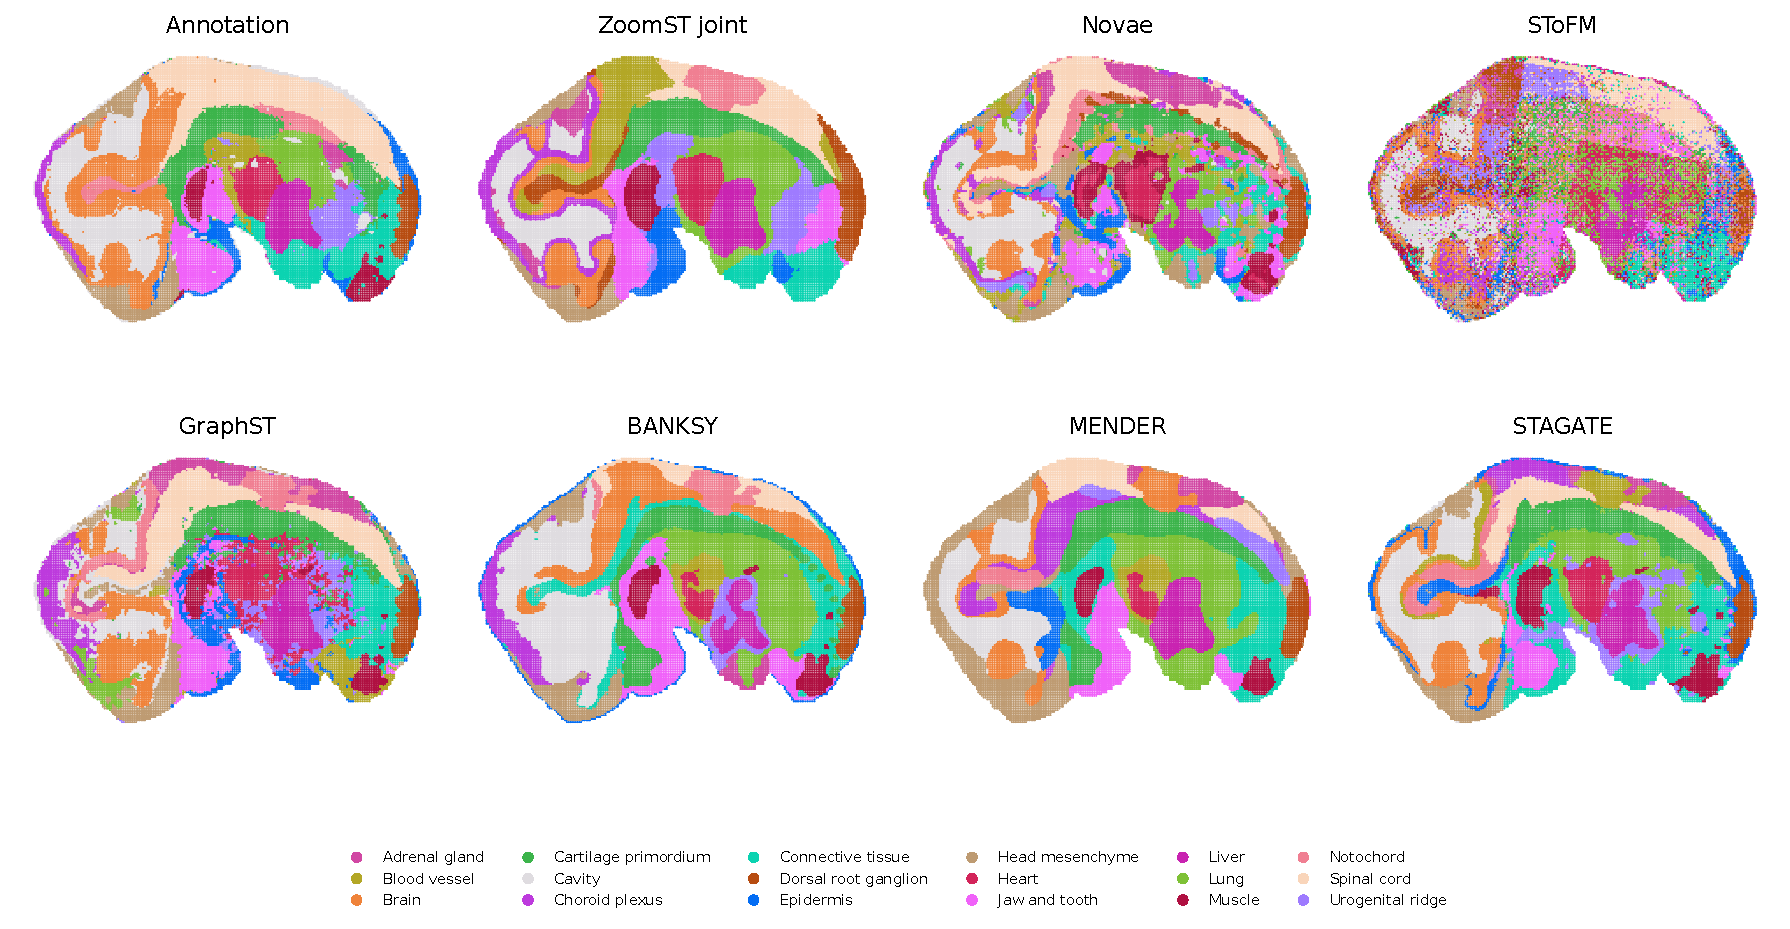
\includegraphics[width=\linewidth]{figures/e125_full_section.pdf}
\caption{\textbf{Example case: whole-section tissue mapping in E12.5 E2S1.} The annotation and seven-method predictions share all 23,640 positions and 18 primary classes. Maximum-overlap one-to-one matching assigns anatomical colors. The top row contains annotation and frozen pretrained features; the lower row contains target-fitted methods. Maps use no smoothing or label interpolation.}
\label{fig:dual-view-e125}
\end{figure}

\begin{figure}[!htbp]
\centering
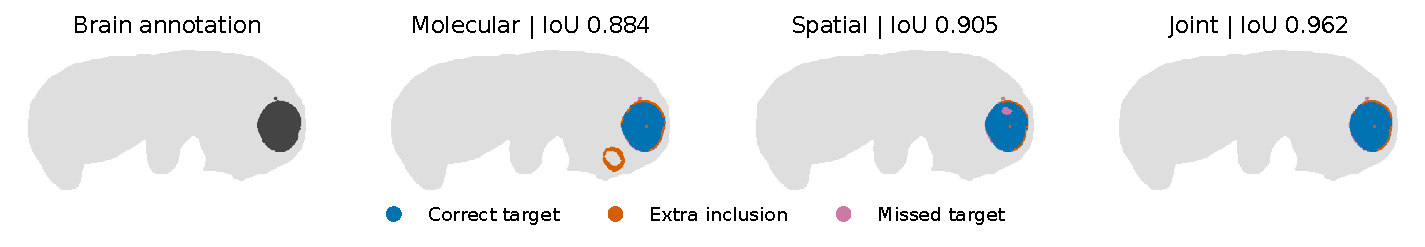
\includegraphics[width=\linewidth]{figures/brain_complementarity.pdf}
\caption{\textbf{Complementary molecular and spatial errors on a held-out section.} Annotation, molecular, spatial, and joint Brain assignments in E16.5 E2S13. Blue: correct assignments; orange: extra assignments; magenta: missed Brain.}
\label{fig:dual-view-brain}
\end{figure}

\begin{figure}[!htb]
\centering
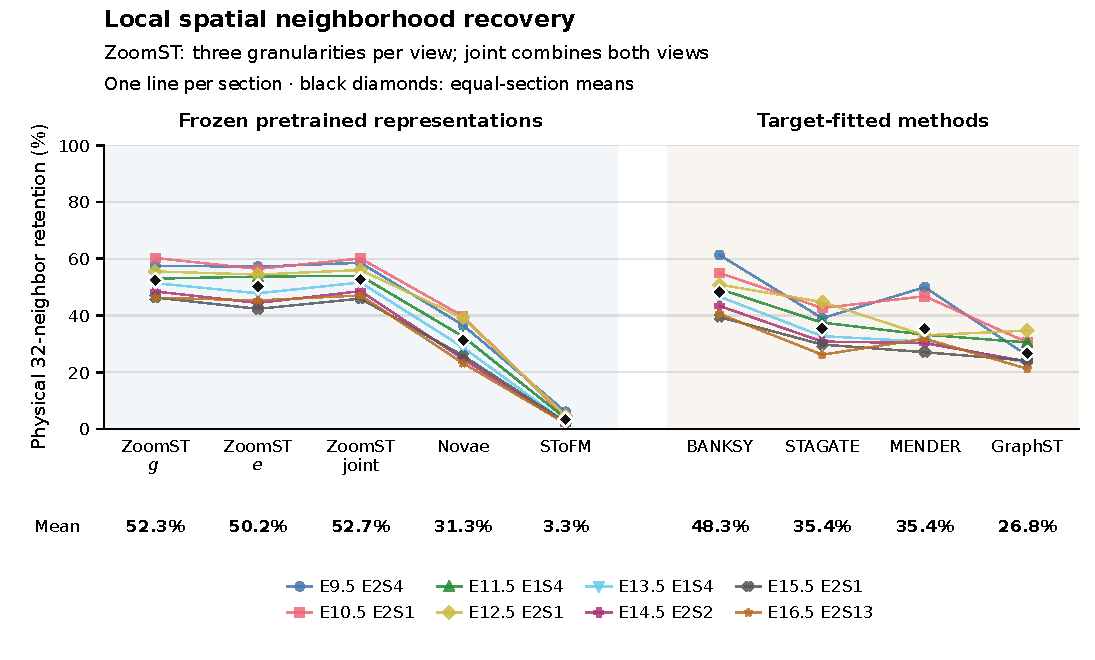
\includegraphics[width=\linewidth]{figures/spatial_retention_multiview.pdf}
\caption{\textbf{Local neighbor retention in the tissue-mapping representations.} Markers show physical 32-neighbor recovery over 2,048 fixed queries per section; all positions are candidates and self is excluded. Colored lines connect the same section within each method group, and black diamonds mark equal-section means. ZoomST $g$ and $e$ each concatenate granularities 8, 32, and 128; joint concatenates both views. All three use the same standardized PCA features as Table~\ref{tab:representation-summary}. Frozen pretrained representations and target-fitted spatial methods are grouped separately.}
\label{fig:dual-view-retention}
\end{figure}

\subsection{Developmental ordering and stage prediction within Brain}
\label{app:developmental-ordering}

MOSTA Brain is selected by coverage across all eight stages and the minimum available stage count. DPT uses the same 589 Brain observations from each held-out section, for 4,712 observations in total. HESTA Brain has sufficient coverage at CS17, CS18, CS19, CS20, and CS23; we fix 512 observations from each section, for 2,560 in total. Models share the same positions within each atlas. ZoomST and No Cross use the frozen models and Joint features defined in Appendix~\ref{app:dual-view}; the cross-method MOSTA comparison additionally uses Novae and SToFM's frozen embeddings and the shared-fit baselines below.

Table~\ref{tab:cross-granularity-development}b evaluates Joint separately at each context size $k\in\{8,32,128\}$. Within each atlas, all six model--scale combinations use the same balanced Brain cohort, 30 neighbors, and a fixed root. Each developmental stage is represented by one held-out section. Table~\ref{tab:joint-scale-comparison} additionally retains the MOSTA whole-section anatomical and physical-neighbor readouts alongside DPT.

\paragraph{Shared representations across sections.}
For the cross-method MOSTA comparison, GraphST and STAGATE each fit one encoder jointly across all eight target sections with shared gene selection and separate within-section spatial graphs. BANKSY uses a common 3,000-gene panel, and MENDER uses a common codebook of 32 unsupervised expression states. These fits use the complete target sections before extracting the balanced Brain observations. Other feature-construction and model-training settings follow Appendix~\ref{app:dual-view}.

\paragraph{Pseudotime.}
External baselines in both atlases share featurewise z-score standardization over the pooled Brain cohort, followed by PCA32 (STAGATE retains its native 30 dimensions). DPT~\citep{haghverdi2016dpt} uses Euclidean neighbor graphs and Scanpy's default distance definition with ten diffusion components.\footnote{\url{https://scanpy.readthedocs.io/en/stable/generated/scanpy.tl.dpt.html}} The default neighborhood size is 30. To address DPT computation failures, we expand the graph to 50 neighbors for STAGATE, BANKSY, and MENDER on MOSTA. Other DPT settings are shared. The MOSTA root is the E9.5 observation nearest the spatial centroid of the sampled E9.5 Brain domain. Sampling and numerical routines use seed 42. Root distances are normalized by the largest finite distance within each method; all selected MOSTA observations have finite pseudotime under the reported settings.

\paragraph{Pseudotime--stage agreement.}
For observation $i$, let $t_i$ denote pseudotime and $s_i$ its measured developmental stage. Spot-level Spearman correlation is $\operatorname{Spearman}(t_i,s_i)$ over all selected observations in an atlas, using unrounded pseudotimes and average ranks for ties. The observations span eight MOSTA stages or five HESTA stages. Figure~\ref{fig:developmental-ordering} reports both atlases; Table~\ref{tab:developmental-ordering} retains the combined-granularity MOSTA values.

For HESTA, the root is the first observation in the sorted sampled CS17 indices, fixed before evaluating the scores; its distances are normalized by the largest finite distance. ZoomST and No Cross have finite pseudotime for all selected Brain observations. Carnegie stage numbers specify the ordered target. PCA and graph construction pool the unlabeled Brain observations within each atlas; stage labels anchor the earliest-stage root and evaluate the resulting order.

\paragraph{HESTA cross-method comparison.}
The HESTA panel uses the same 2,560 Brain observations and CS17 root. Frozen external representations comprise Novae, SToFM, scGPT-spatial, the Cell, Neighborhood, and Spatial-cell outputs of TERRA, and CellWorld. They follow the standardization and DPT protocol above, with 30 neighbors for every method. CellWorld uses its frozen CP10K/log1p and per-section Seurat-HVG300 export. Its 512 CS18 observations are disconnected from the common root, so the figure marks its complete-stage readout as NA. The remaining methods cover all five stages. The existing independently fitted per-section DECIPHER embeddings are not pooled into a shared cross-stage coordinate system.

\begin{table}[!htbp]
\centering\scriptsize
\caption{\textbf{MOSTA Joint readouts by granularity.} AMI means follow Table~\ref{tab:cross-granularity-ami}a; SD is the sample SD across three downstream clustering runs. Neighbor retention is equal-section physical 32-neighbor recovery. Spot-level correlation uses the 4,712-observation Brain cohort. Bold marks the higher value in each pair, including ties.}
\label{tab:joint-scale-comparison}
\setlength{\tabcolsep}{2.2pt}
\renewcommand{\arraystretch}{1.18}
\begin{tabular}{l*{9}{c}}
\toprule
 & \multicolumn{3}{c}{AMI $\uparrow$} & \multicolumn{3}{c}{Neighbor retention (\%) $\uparrow$} & \multicolumn{3}{c}{Spot-level $\rho\uparrow$} \\
\cmidrule(lr){2-4}\cmidrule(lr){5-7}\cmidrule(lr){8-10}
Model & 8 & 32 & 128 & 8 & 32 & 128 & 8 & 32 & 128 \\
\midrule
ZoomST & \textbf{0.585 $\pm$ 0.006} & \textbf{0.571 $\pm$ 0.003} & 0.538 $\pm$ 0.002 & \textbf{35.1} & \textbf{52.7} & \textbf{62.5} & 0.868 & \textbf{0.822} & \textbf{0.354} \\
No Cross & 0.570 $\pm$ 0.001 & 0.562 $\pm$ 0.005 & \textbf{0.539 $\pm$ 0.0003} & 34.2 & 50.5 & 61.4 & \textbf{0.903} & 0.738 & -0.239 \\
\bottomrule
\end{tabular}

\end{table}

\begin{table}[!htbp]
\centering\small
\caption{\textbf{Spot-level pseudotime--stage Spearman correlation within Brain.} Correlation is computed over all 4,712 observations spanning eight MOSTA stages. Bold marks the highest value.}
\label{tab:developmental-ordering}
\setlength{\tabcolsep}{10pt}
\renewcommand{\arraystretch}{1.05}
\begin{tabular}{lc}
\toprule
Representation & \shortstack{Spot-level\\Spearman $\rho$} \\
\midrule
ZoomST joint & \textbf{0.816} \\
Novae & 0.714 \\
SToFM & 0.341 \\
ZoomST no cross & 0.651 \\
GraphST & 0.491 \\
STAGATE & 0.229 \\
BANKSY & -0.267 \\
MENDER & 0.458 \\
\bottomrule
\end{tabular}

\end{table}

\paragraph{Developmental-stage prediction.}
The linear probe uses the original Joint features without PCA. Each leave-one-section-out fold fits StandardScaler and a Ridge regressor only on Brain observations from the remaining sections. The intercept is unpenalized and the Ridge coefficient is $\alpha=n_{\mathrm{train}}\lambda$, with fixed $\lambda=0.1$. MOSTA training folds use 512 Brain observations per section and evaluate every Brain observation in the test section. HESTA uses the same fixed 512-observation-per-section cohort for training and testing across folds. Targets are embryonic days for MOSTA and Carnegie stages for HESTA. Encoder weights remain frozen throughout.

For section $s$ with $n_s$ evaluated observations, $\mathrm{MAE}_s=n_s^{-1}\sum_i|\hat{s}_i-s|$; reported MAE averages the included sections equally. Relative reduction is $(\overline{\mathrm{MAE}}_{\mathrm{No\ Cross}}-\overline{\mathrm{MAE}}_{\mathrm{ZoomST}})/\overline{\mathrm{MAE}}_{\mathrm{No\ Cross}}$.
\FloatBarrier


\section{Cross-granularity prediction}
\label{app:granularity-transfer}

\paragraph{Representation states.}
The final MOSTA model specified in Section~\ref{sec:experiments} supplies native 256-dimensional molecular states without standardization. Data use follows Table~\ref{tab:evaluation_protocol}.

\paragraph{Same-location state prediction.}
For every position in each section, define $m_i^T=d^{-1}\|T_{a\to b}(e_{i,a})-e_{i,b}\|_2^2$ and $m_i^0=d^{-1}\|e_{i,a}-e_{i,b}\|_2^2$. Figure~\ref{fig:granularity-transfer}A reports $\rho_{ab}=\sum_i m_i^T/\sum_i m_i^0$ for each section. The unchanged source is the no-transformation reference; the target is directly encoded from the actual broader neighborhood at the same location. Improved-position fractions use $n^{-1}\sum_i\mathbf 1[m_i^T<m_i^0]$. Scores are computed over all positions in each evaluated section. This evaluation differs from training, where all centers within each coarse support contribute sources.

\paragraph{Projected joint association.}
Each section supplies the same fixed 2,048 positions, partitioned into four disjoint batches of 512. For each batch, correct predicted pairings, unchanged-source controls, and 20 shuffled predictions are compared with directly encoded fine--coarse pairs. Each shuffle has no fixed points and permutes only predicted destinations, preserving their marginal distribution. The product kernel uses source and target bandwidths from the corresponding observed states, shared across controls, with the settings in Appendix~\ref{app:hyperparameters}.

We evaluate the checkpoint's training projection and eight fixed orthogonal projections with seeds 2026091501--2026091508. Figure~\ref{fig:granularity-transfer}B divides the mean correct-pair MMD by the mean shuffled MMD after averaging batches and the eight fresh projections within each section. Correct pairing improves on shuffling in all 864 batch--projection--direction conditions. Compared with the unchanged source on the training projection, transformation lowers joint discrepancy in 21 of 24 section--direction conditions. All three exceptions are in E12.5 E2S1; its projected joint discrepancy increases for each training direction. Table~\ref{tab:granularity-transfer-sections} reports every section and direction.

\begin{figure}[!htbp]
\centering
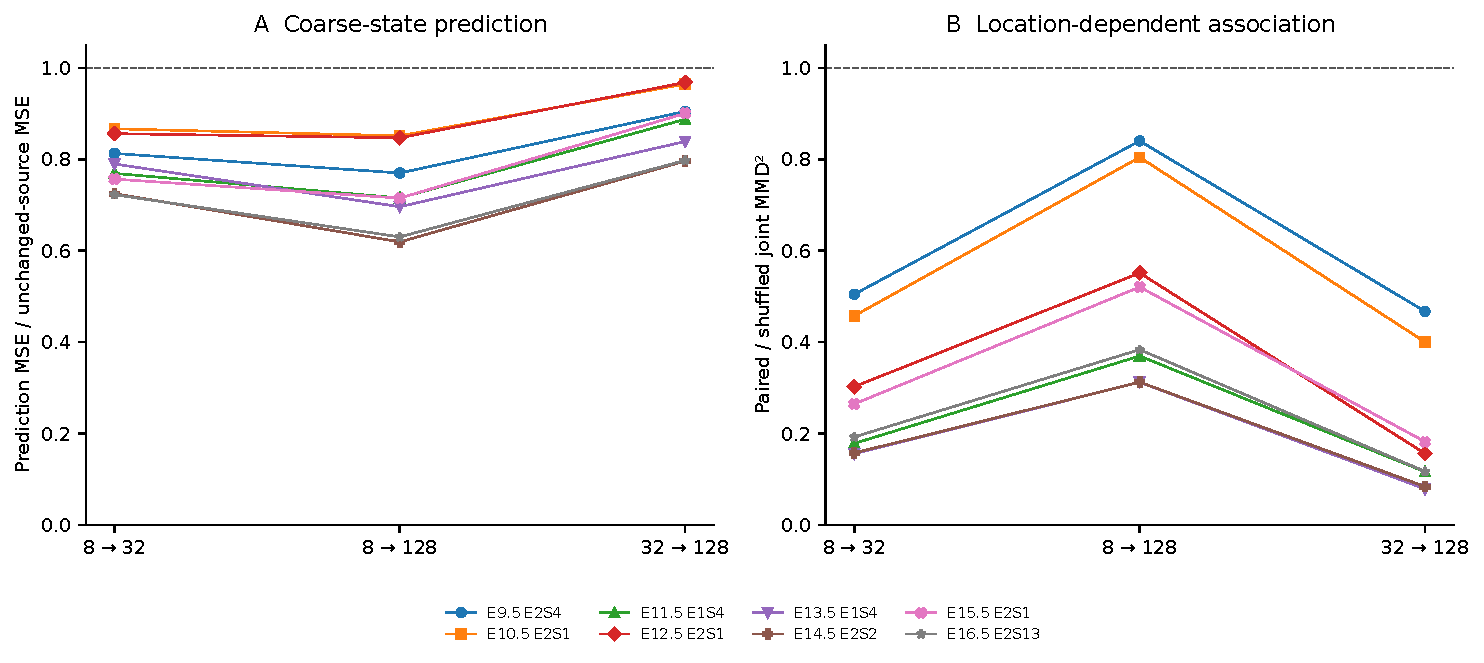
\includegraphics[width=\linewidth]{figures/granularity_transfer.pdf}
\caption{\textbf{Predictive relationships across held-out tissue sections.} \textbf{A}, Target-MSE ratio of transformed to untransformed fine states, using the same directly encoded coarse reference. \textbf{B}, Joint-MMD ratio of correct to shuffled predicted pairings, averaged over four batches and eight projections unused in training. Each line denotes one section; values below one favor the learned prediction or correct pairing.}
\label{fig:granularity-transfer}
\end{figure}

\begin{table}[!htbp]
\centering\small
\caption{\textbf{Coarse-state prediction on every held-out section.} MSE ratio compares transformed and unchanged sources against the same encoded coarse target. Improved is the percentage of positions with lower MSE. Paired/shuffled is the joint-MMD ratio averaged over batches and fresh projections.}
\label{tab:granularity-transfer-sections}
\begin{tabular}{lcccc}
\toprule
Section & Pair & MSE ratio & Improved (\%) & Paired/shuffled \\
\midrule
E9.5 E2S4 & 8$\to$32 & 0.813 & 98.0 & 0.505 \\
E9.5 E2S4 & 32$\to$128 & 0.905 & 84.3 & 0.467 \\
E9.5 E2S4 & 8$\to$128 & 0.770 & 98.3 & 0.840 \\
E10.5 E2S1 & 8$\to$32 & 0.867 & 88.7 & 0.458 \\
E10.5 E2S1 & 32$\to$128 & 0.965 & 58.7 & 0.400 \\
E10.5 E2S1 & 8$\to$128 & 0.851 & 88.7 & 0.804 \\
E11.5 E1S4 & 8$\to$32 & 0.769 & 97.9 & 0.178 \\
E11.5 E1S4 & 32$\to$128 & 0.888 & 82.3 & 0.116 \\
E11.5 E1S4 & 8$\to$128 & 0.715 & 98.2 & 0.370 \\
E12.5 E2S1 & 8$\to$32 & 0.856 & 88.9 & 0.302 \\
E12.5 E2S1 & 32$\to$128 & 0.968 & 53.7 & 0.156 \\
E12.5 E2S1 & 8$\to$128 & 0.847 & 84.1 & 0.551 \\
E13.5 E1S4 & 8$\to$32 & 0.790 & 97.4 & 0.156 \\
E13.5 E1S4 & 32$\to$128 & 0.839 & 89.0 & 0.079 \\
E13.5 E1S4 & 8$\to$128 & 0.696 & 98.5 & 0.312 \\
E14.5 E2S2 & 8$\to$32 & 0.725 & 98.6 & 0.157 \\
E14.5 E2S2 & 32$\to$128 & 0.796 & 91.9 & 0.084 \\
E14.5 E2S2 & 8$\to$128 & 0.619 & 99.5 & 0.312 \\
E15.5 E2S1 & 8$\to$32 & 0.757 & 93.9 & 0.265 \\
E15.5 E2S1 & 32$\to$128 & 0.900 & 59.2 & 0.182 \\
E15.5 E2S1 & 8$\to$128 & 0.715 & 91.7 & 0.521 \\
E16.5 E2S13 & 8$\to$32 & 0.722 & 97.9 & 0.192 \\
E16.5 E2S13 & 32$\to$128 & 0.798 & 91.4 & 0.117 \\
E16.5 E2S13 & 8$\to$128 & 0.630 & 98.3 & 0.383 \\
\bottomrule
\end{tabular}

\end{table}


\clearpage
\section{Unseen granularities and context response}
\label{app:scale-continuum}

\paragraph{Figure~\ref{fig:granularity-query-summary}: evaluation and aggregation.}
All three panels use eight sections excluded from pretraining, with the encoder and transformation frozen. In panels (a,b), target MSE compares unchanged source states and ZoomST predictions against the same directly encoded targets. Panel (a) averages the trained pairs $8\to32$, $8\to128$ and $32\to128$ within each section, using all section positions. Panel (b) averages the six unseen targets $12,16,24,48,64,96$ queried from $e_8$ at 1,024 fixed positions per section. Panel (c) selects the lowest and highest predicted-response quarters separately within each section and doubling interval ($8\to16$, $16\to32$, $32\to64$, $64\to128$), with 256 locations per quarter, then averages their directly encoded changes over the four intervals. Each box therefore contains eight section means. The highest-response quarter shows larger encoded changes than the lowest quarter in 31 of 32 section--interval conditions (Figure~\ref{fig:granularity-query-summary}c).

\subsection{Transition heads on a shared frozen encoder}
\label{app:transition-comparison}

\paragraph{Shared-encoder comparison.}
The neural ODE and granularity-conditioned residual MLP are trained at 8, 32 and 128 on a shared frozen encoder, then evaluated against the same directly encoded targets. Averaging MSE over six unseen granularities, the ODE reduces error on every held-out section, with a mean paired reduction of 10.86\% (Figure~\ref{fig:ode-transition-comparison}).

\begin{figure}[!htbp]
\centering
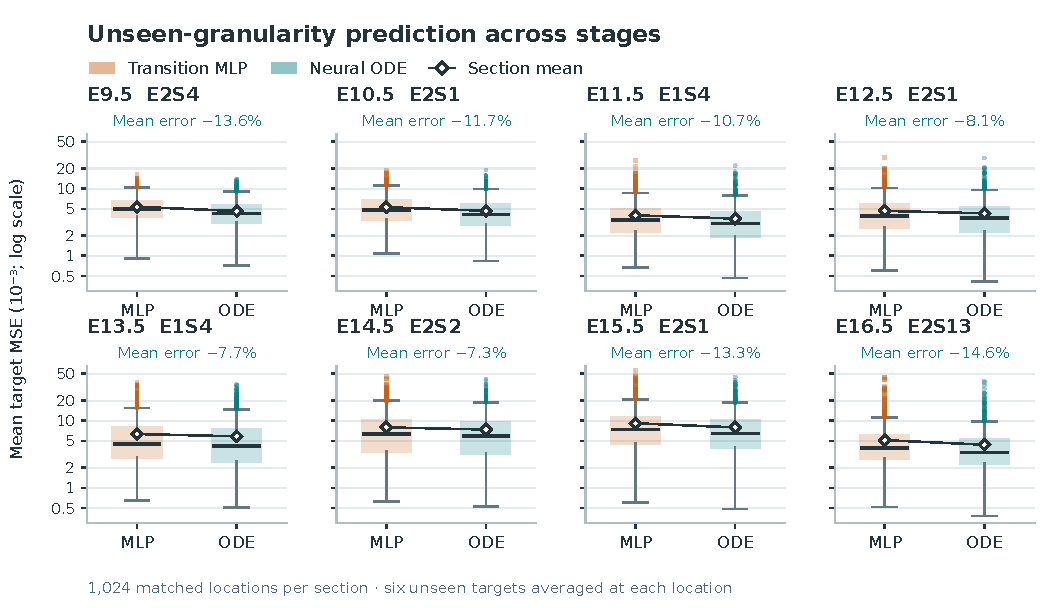
\includegraphics[width=\linewidth]{figures/ode_vs_transition_boxplots.pdf}
\caption{\textbf{Lower mean unseen-granularity error with neural ODE.} Each panel compares the granularity-conditioned residual MLP and ODE on one held-out section. Both heads use the same frozen encoder, fine-state inputs and directly encoded targets. Each box contains 1,024 location-level MSEs, each averaged equally over $k\in\{12,16,24,48,64,96\}$. Boxes show medians and interquartile ranges; whiskers extend to 1.5 interquartile ranges, with all outliers shown. Connected diamonds mark section means; percentages give their paired relative reductions. All panels share the same logarithmic axis.}
\label{fig:ode-transition-comparison}
\end{figure}

We compare the ODE with the granularity-conditioned residual MLP,
\[
T^{\mathrm{MLP}}_{a\to b}(z)=z+\mathrm{MLP}\!\left([\mathrm{LN}(z),h(a),h(b),u(b)-u(a)]\right).
\]
The MLP has dimensions $321\to128\to256$ with GELU activation and 32-dimensional scale embeddings; the ODE field has dimensions $257\to128\to256$. For a query between adjacent trained coordinates $u_j,u_{j+1}$, the MLP uses $h(k)=(1-w)h_j+wh_{j+1}$ with $w=(u(k)-u_j)/(u_{j+1}-u_j)$. The heads contain 74,848 and 66,560 trainable parameters, respectively.

Both heads are initialized afresh and trained on the same frozen encoder outputs from all 45 source sections for two epochs (7,224 updates; batch 1,024). AdamW uses learning rate $2\times10^{-4}$, 188 warmup steps and cosine decay to one tenth of the peak rate; gradient norms are clipped at five. Weight decay is 0.02 for weight matrices, 0.01 for scale embeddings and zero for normalization and bias terms. The ODE uses RK4 with maximum step 0.25 in $u$. Evaluation uses the same 1,024 positions per held-out section and the same directly encoded targets for both heads.

For section $s$, let $M_s^m$ be its MSE averaged equally over the six unseen targets for head $m$. The mean paired reduction is $100\,\mathrm{mean}_s(1-M_s^{\mathrm{ODE}}/M_s^{\mathrm{MLP}})=10.86\%$, ranging from 7.28\% to 14.56\% across sections. Table~\ref{tab:ode-transition-frozen} gives the section summaries underlying Figure~\ref{fig:ode-transition-comparison}. These are separately fitted transition heads on a common reference encoder.

\begin{table}[!htbp]
\centering\small
\caption{\textbf{Matched transition heads on a shared frozen encoder.} MSE is averaged over all six unseen targets and 1,024 locations per section. The mean reduction averages the eight paired section reductions.}
\label{tab:ode-transition-frozen}
\begin{tabular}{lccc}
\toprule
Section & MLP MSE ($\times10^{-3}$) & ODE MSE ($\times10^{-3}$) & Reduction (\%) \\
\midrule
E9.5 E2S4 & 5.381 & 4.650 & 13.57 \\
E10.5 E2S1 & 5.303 & 4.682 & 11.73 \\
E11.5 E1S4 & 4.014 & 3.585 & 10.69 \\
E12.5 E2S1 & 4.673 & 4.295 & 8.08 \\
E13.5 E1S4 & 6.342 & 5.853 & 7.71 \\
E14.5 E2S2 & 7.971 & 7.391 & 7.28 \\
E15.5 E2S1 & 9.174 & 7.957 & 13.26 \\
E16.5 E2S13 & 5.140 & 4.392 & 14.56 \\
Mean & 6.000 & 5.350 & 10.86 \\
\bottomrule
\end{tabular}

\end{table}

\subsection{Agreement with unseen neighborhood encodings}
\label{app:unseen-state-detail}

\paragraph{Frozen state prediction.}
The MOSTA encoder and ODE transition are frozen after joint training at 8,32,128. We use 1,024 fixed positions on each of the eight held-out sections and directly encode neighborhoods at $\mathcal K=\{8,12,16,24,32,48,64,96,128\}$. The molecular encoding procedure and neighborhood ordering remain unchanged. All predictions start from the same $e_{i,8}$; the encoded intermediate states are scoring references and do not enter these predictions.

Let $\widehat e_i(k)=T_{8\to k}(e_{i,8})$ and $\mathcal U=\mathcal K\setminus\{8,32,128\}$. For section $s$, target MSE averages $d^{-1}\|\widehat e_i(k)-e_i(k)\|^2$ over positions. The section's relative gain is one minus its MSE averaged over $k\in\mathcal U$ divided by the corresponding unchanged-$e_8$ MSE. Gains are then averaged over eight sections, yielding 21.96\%. Normalized RMSE divides RMSE by the target's root-mean-square variation around its section mean, so $R^2=1-\mathrm{NRMSE}^2$ within each section. Prediction improves over unchanged $e_8$ in all 48 section--target conditions. Figure~\ref{fig:granularity-query-summary}b plots absolute MSE averaged over the six targets within each section, giving eight paired section means.

\paragraph{Distance to a common directly encoded target.}
For the direct-distance comparison in Figure~\ref{fig:ode-unseen-distance-distributions}, define
\[
d_i^{\mathrm{start}}(k)=\frac{\|e_{i,8}-e_i(k)\|_2}{\sqrt d},\qquad
d_i^{\mathrm{pred}}(k)=\frac{\|\widehat e_i(k)-e_i(k)\|_2}{\sqrt d}.
\]
At each target, we average these per-position RMS distances within each section. Sections receive equal weight in the summary. Averaging $1-\overline d_s^{\mathrm{pred}}(k)/\overline d_s^{\mathrm{start}}(k)$ equally over the six unseen targets and eight sections gives a 10.38\% reduction, ranging from 3.04\% to 20.55\% across the 48 conditions. Every condition has a lower mean and median prediction distance. Within individual conditions, 81.15--99.71\% of positions are closer to the target. This RMS-distance statistic differs from the reduction in mean squared error reported above.

\begin{figure}[!htbp]
\centering
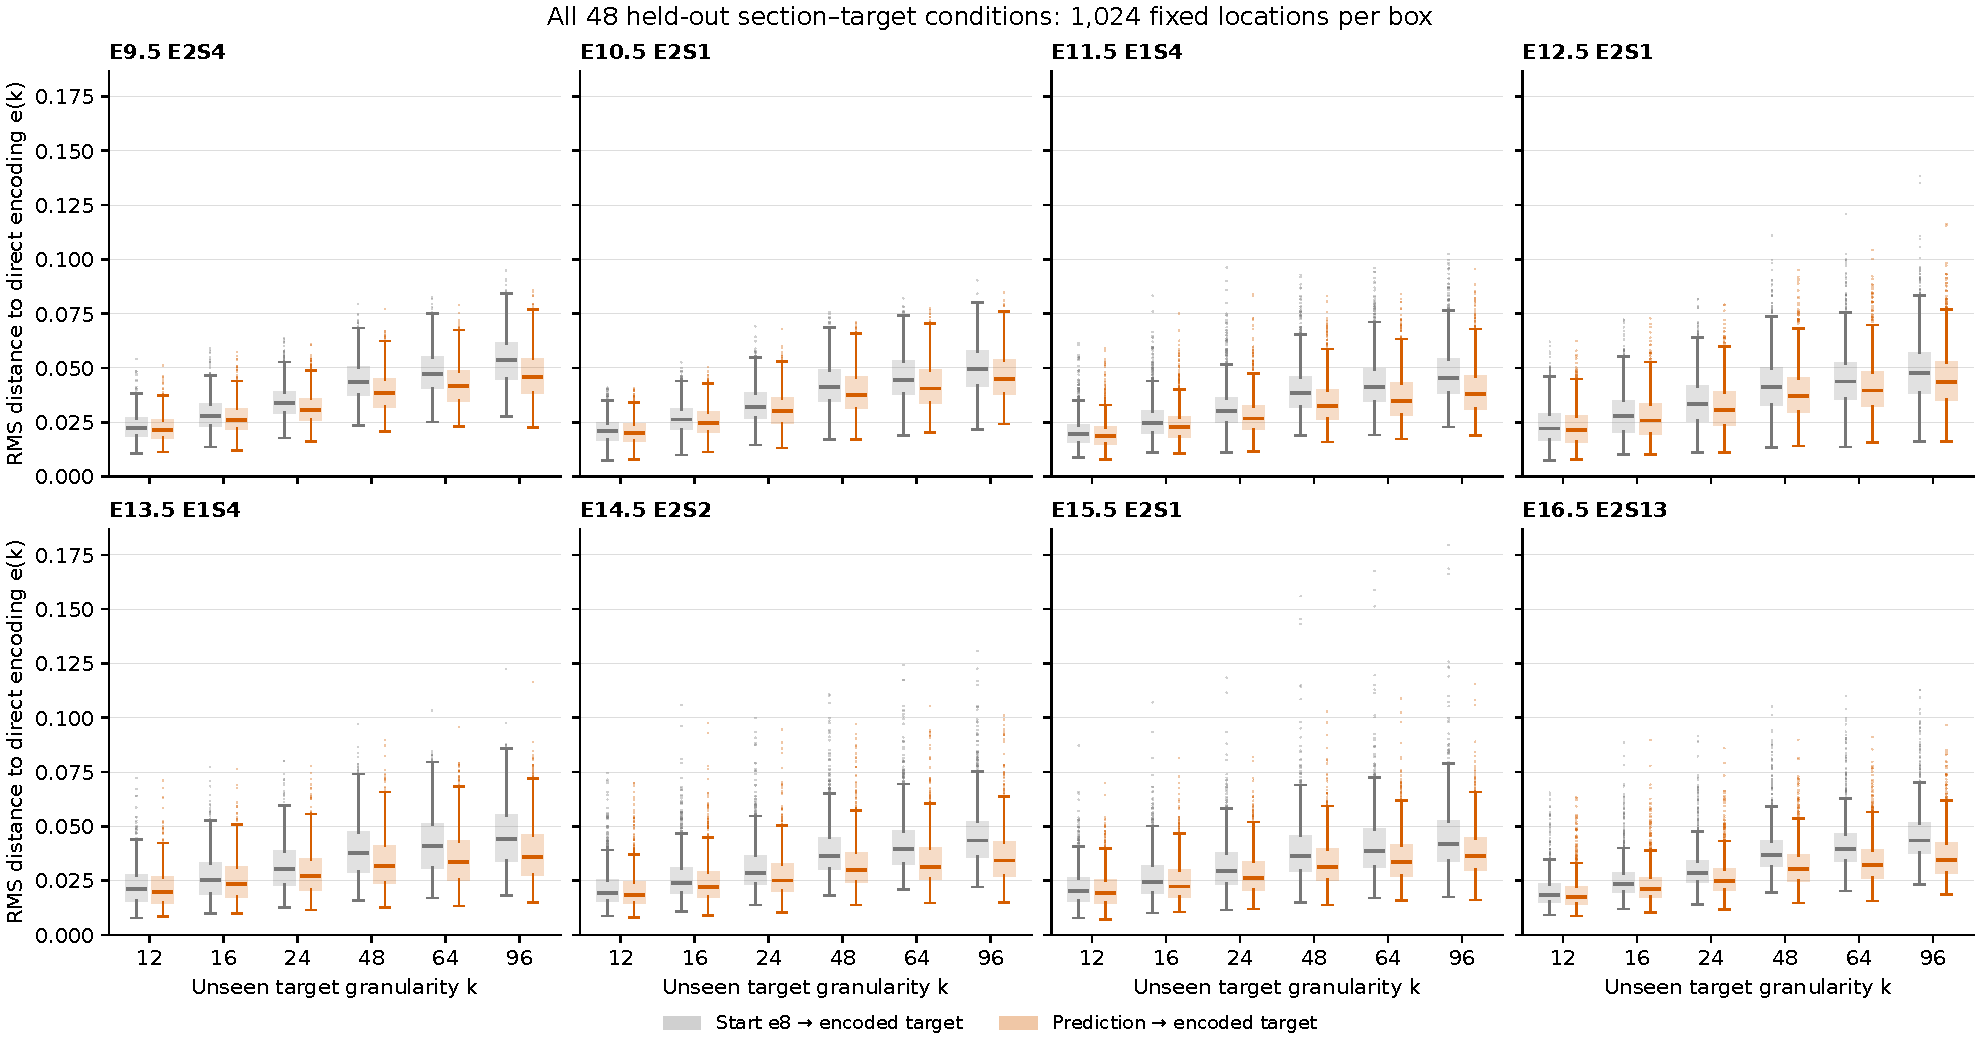
\includegraphics[width=\linewidth]{figures/unseen_state_distances_all_sections.pdf}
\caption{\textbf{Within-section distributions of distance to directly encoded unseen states.} The panels cover eight held-out sections and six unseen target granularities. Each pair compares distances from unchanged $e_8$ and from the prediction to the same target at the same 1,024 fixed positions. Boxes show medians and interquartile ranges, whiskers extend to 1.5 interquartile ranges, and outliers are retained. Position distributions describe each section; section means are the units in the main comparison.}
\label{fig:ode-unseen-distance-distributions}
\end{figure}

\paragraph{Shared-space visualization and full-state error.}
The E16.5 E1S1 analysis uses 1,024 fixed positions. We fit a center-only, full-SVD PCA on the directly encoded states at all nine granularities, then apply the same mean and components to predictions. All positions are shown with common axis limits. The first two PCs explain 20.25\% and 17.02\% of encoded-state variance. Table~\ref{tab:ode-case-pca} reports prediction accuracy in the full 256-dimensional space.

\begin{figure}[!htbp]
\centering
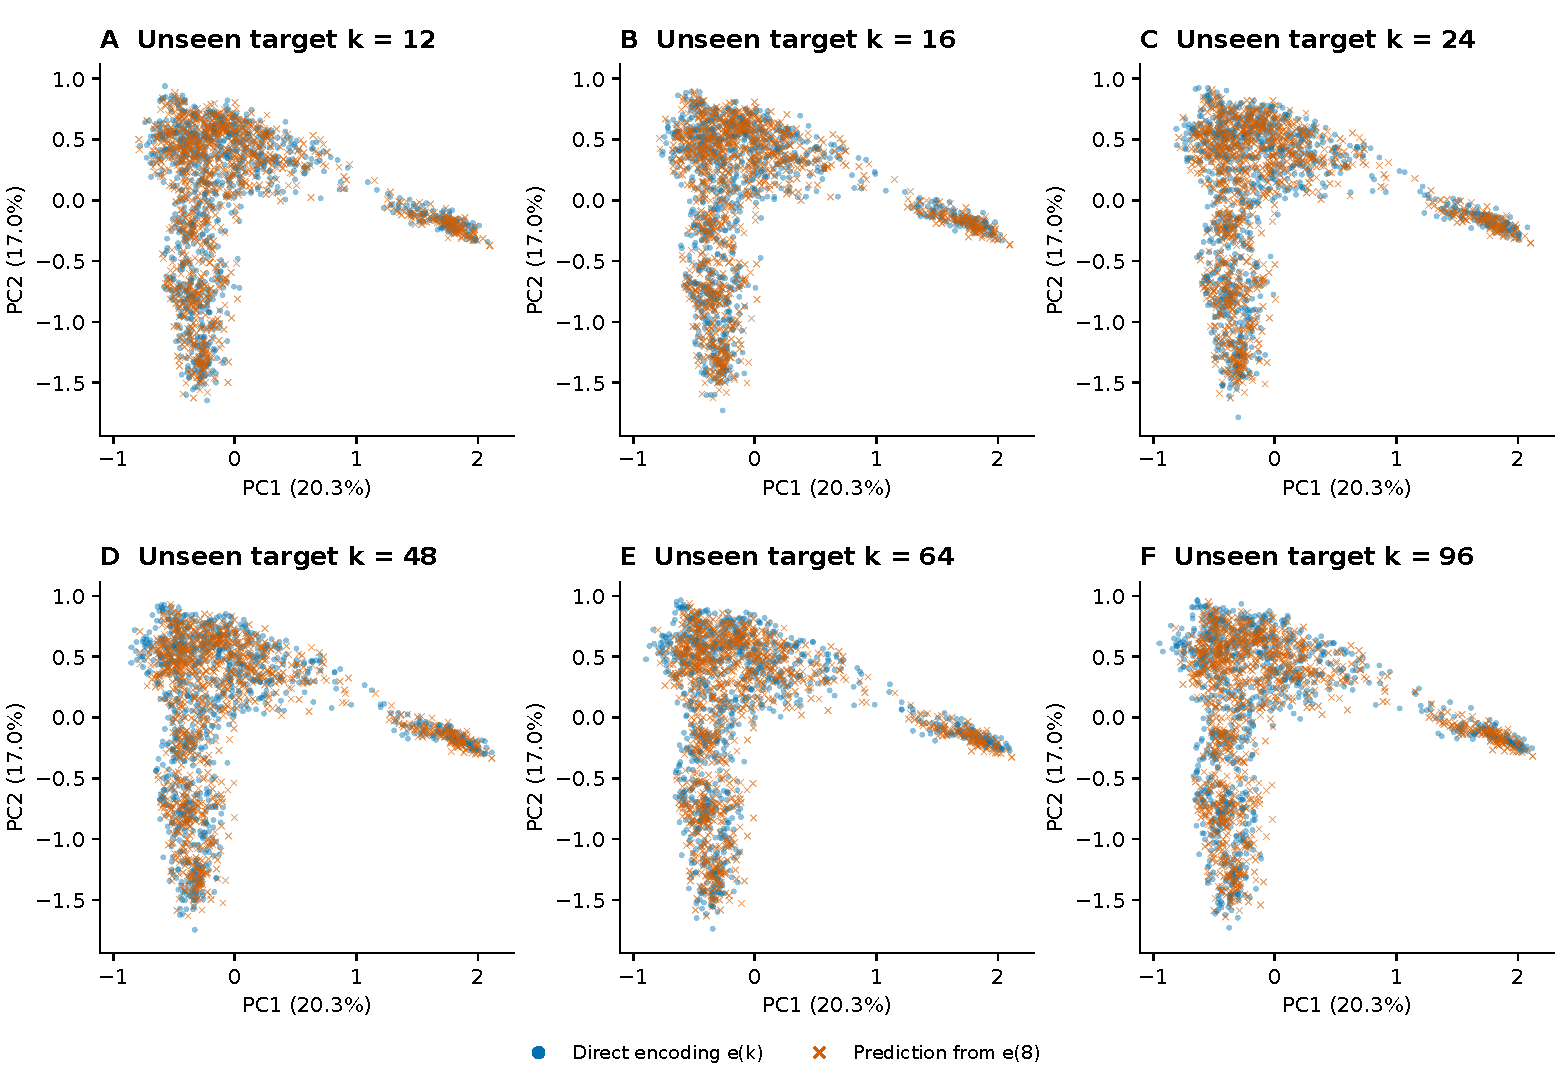
\includegraphics[width=\linewidth]{figures/case_all_unseen_pca_no_pair_lines.pdf}
\caption{\textbf{All six unseen target states in the E16.5 E1S1 case.} Every panel uses the same PCA basis and the same 1,024 positions. Metrics are computed in 256 dimensions. Targets and predictions are paired at each location.}
\label{fig:ode-case-all-pca}
\end{figure}
\begin{table}[!htbp]
\centering\small
\caption{\textbf{Full-dimensional accuracy underlying the case PCA.} MSE ratio compares prediction with unchanged $e_8$ against directly encoded targets; NRMSE and $R^2$ use the same full-dimensional targets.}
\label{tab:ode-case-pca}
\begin{tabular}{lccc}
\toprule
Target $k$ & MSE ratio & NRMSE & $R^2$ \\
\midrule
12 & 0.884 & 0.206 & 0.958 \\
16 & 0.810 & 0.243 & 0.941 \\
24 & 0.739 & 0.280 & 0.922 \\
48 & 0.664 & 0.333 & 0.889 \\
64 & 0.643 & 0.352 & 0.876 \\
96 & 0.621 & 0.377 & 0.858 \\
\bottomrule
\end{tabular}

\end{table}

\FloatBarrier
\subsection{Context-response evaluation across observation ranges}
\label{app:response-meaning}

\paragraph{Matched response definitions and sampling.}
For $\widehat e_i(k)=T_{8\to k}(e_{i,8})$, Figure~\ref{fig:granularity-query-summary}c, Figure~\ref{fig:ode-context}a and the grouping in Figure~\ref{fig:facial-nerve-composition} use
\[
D_i^{\mathrm{pred}}(a,b)=
\frac{\|\widehat e_i(b)-\widehat e_i(a)\|_2}{\sqrt d\,\log_2(b/a)},\qquad
D_i^{\mathrm{enc}}(a,b)=
\frac{\|e_i(b)-e_i(a)\|_2}{\sqrt d\,\log_2(b/a)}.
\]
Both operands in the predicted displacement belong to queries from the same fixed $e_8$. Encoded states are evaluation references, and all displayed doubling intervals have log width one.

Held-out comparisons use 1,024 fixed locations per section. Anatomical cases use the training sections identified in Table~\ref{tab:evaluation_protocol}, with up to 128 locations per annotation selected by a fixed hash of observation identity; smaller domains retain every location.

\paragraph{Held-out location ordering.}
For each held-out section and each doubling interval, we sort the 1,024 locations by predicted response and split them into four equal groups; ties preserve sample order. We compare the directly encoded changes in the lowest and highest quarters. Figure~\ref{fig:granularity-query-summary}c averages these group means over the four intervals within each section, giving eight paired section means.

\paragraph{Actual neighborhood composition.}
Let $q_{ic}(k)$ be the proportion of annotation $c$ among the $k-1$ neighbors after excluding the focal center. For the same interval as the response,
\[
C_i(a,b)=\tfrac12\sum_c|q_{ic}(b)-q_{ic}(a)|.
\]
Support ordering is identical to the model input, and unknown-label mass is retained. The Facial nerve composition bars (Figure~\ref{fig:facial-nerve-composition}) follow the same 16 locations in each extreme predicted-response quarter. Their mean encoded changes are 0.0191 and 0.0343 in the low and high groups, respectively (ratio 1.799). Corresponding mean TV values are 0.134 and 0.284. Composition TV quantifies the change in annotated tissue proportions.

\begin{figure}[!htbp]
\centering
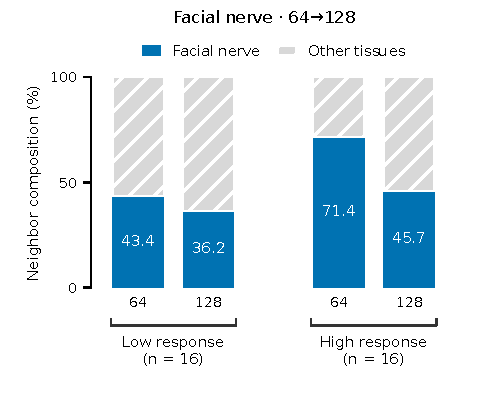
\includegraphics[width=0.58\linewidth]{figures/facial_nerve_composition.pdf}
\caption{\textbf{Neighborhood composition in low- and high-response Facial nerve locations.} The groups are the lowest and highest predicted-response quarters among all 64 Facial nerve locations in the E14.5 E1S1 training section, using the $64\to128$ response in Figure~\ref{fig:ode-context}a. Each pair of bars follows the same 16 locations at both granularities. Blue shows the mean Facial nerve fraction; gray shows all other labels. Predictions start from fixed $e_8$.}
\label{fig:facial-nerve-composition}
\end{figure}

\paragraph{Within-Brain changes under a constant annotation.}
Among sampled Brain locations whose neighborhoods remain entirely Brain-labeled at both $r=8$ and $r=16$, predicted responses correlate with directly encoded changes (Spearman $\rho=0.645$), showing molecular-context variation within a constant anatomical annotation.

\paragraph{Whole-section spatial overview.}
Figure~\ref{fig:ode-context}b averages the instantaneous response $s_i(2^t)=\|f_\theta(z_i((t-3)/4),(t-3)/4)\|_2/(4\sqrt d)$ over 64 equally spaced midpoints in $t=\log_2 k\in[3,7]$. This path average differs from the finite response used in panel (a) and to define the groups in Figure~\ref{fig:facial-nerve-composition}. Colors use an empirical percentile reference pooled over the full-range mean and the four doubling-range means, with all 121,767 locations included. Panel (c) shows observed composition TV from 8 to 128. The maps show spatial distributions without smoothing; their whole-section Spearman correlation is 0.174. Both maps are rotated together by $180^\circ$ relative to the source coordinates for display, preserving distances and the common orientation. Spatial scale bars use the nominal $25\,\mu$m pitch of the bin50 matrices~\citep{chen2022mosta}; response remains normalized by $\log_2 k$.


\clearpage
\section{Objective ablation on MOSTA}
\label{app:objective-ablation}

We compare No Cross, CS, and ZoomST using a common initialization, the same training data and training budget, and identical training settings apart from the loss terms. No Cross uses within-granularity learning; CS adds coarse-support supervision; ZoomST further adds JointMMD. Evaluation uses frozen encoders and the held-out MOSTA split from Section~\ref{sec:developmental-information}, with identical evaluation observations and readout settings across the three models. All readouts use Joint representations at granularities 8, 32, and 128.

Table~\ref{tab:mosta-objective-ablation} follows the anatomical clustering, Brain developmental ordering, and stage-prediction protocols in Appendix~\ref{app:dual-view}--\ref{app:developmental-ordering}.

Adding JointMMD to CS reduces stage-prediction MAE and increases spot-level DPT correlation at all three granularities, with the largest gains at granularity 128. AMI increases at granularities 8 and 32 and remains similar at granularity 128.

\begin{table}[!htbp]
\centering
\caption{\textbf{Controlled objective ablation on MOSTA.} Joint AMI, Brain spot-level DPT--stage Spearman correlation, and Brain stage-prediction MAE. AMI averages the eight held-out sections equally; $\pm$ denotes SD over downstream clustering runs. DPT and stage MAE use the protocols and aggregation of Table~\ref{tab:cross-granularity-development}b. Bold marks the best unrounded mean in each column.}
\label{tab:mosta-objective-ablation}
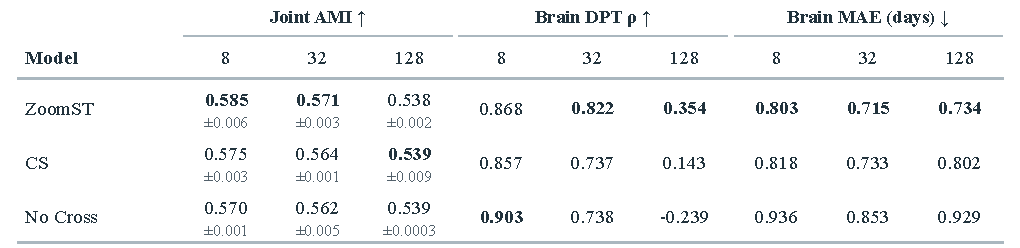
\includegraphics[width=\linewidth]{figures/mosta_objective_ablation.pdf}
\end{table}
\FloatBarrier

